\documentclass[border=6pt]{standalone}
\usepackage{fontspec}
\IfFileExists{fonts/times.ttf}{
  \setmainfont{times.ttf}[Path=fonts/,
    BoldFont=timesbd.ttf, ItalicFont=timesi.ttf, BoldItalicFont=timesbi.ttf]
}{\usepackage{mathptmx}}
\usepackage{tikz}
\usetikzlibrary{arrows.meta,positioning,fit,backgrounds,calc,shapes.geometric}
\begin{document}
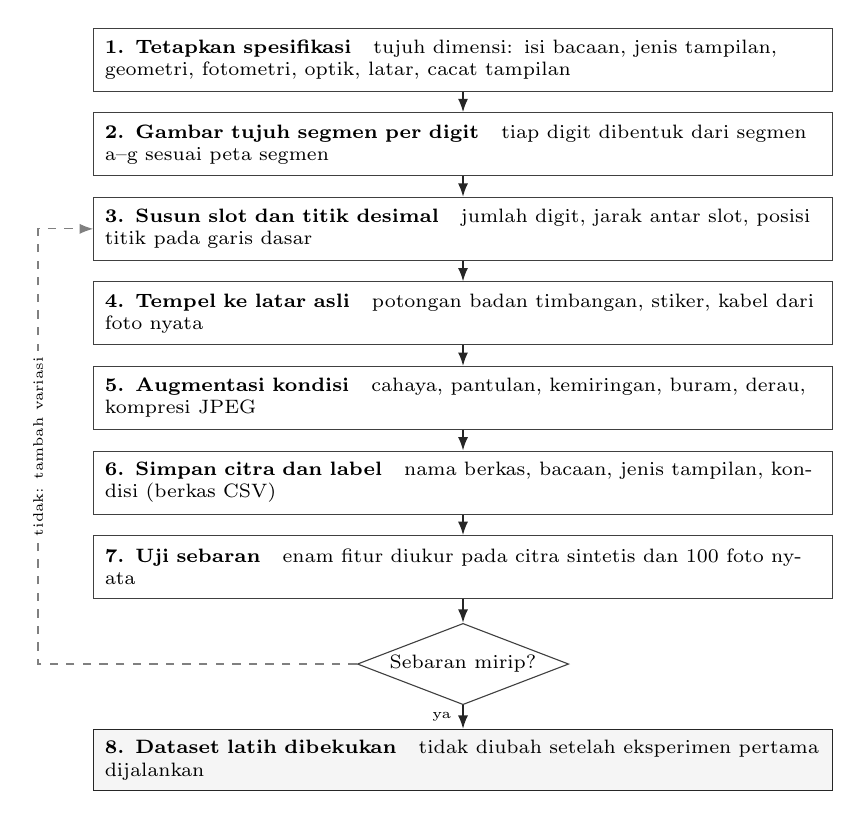
\begin{tikzpicture}[
  x=1cm, y=1cm,
  langkah/.style={rectangle, draw=black!75, fill=white, align=left,
                  text width=9.1cm, minimum height=0.80cm, inner sep=4pt,
                  font=\scriptsize},
  kunci/.style={rectangle, draw=black!85, fill=black!4, align=left,
                text width=9.1cm, inner sep=4pt, font=\scriptsize},
  tanya/.style={diamond, draw=black!75, fill=white, aspect=2.6,
                align=center, font=\scriptsize, inner sep=1pt},
  panah/.style={-{Latex[length=1.7mm]}, draw=black!85, semithick},
  balik/.style={-{Latex[length=1.7mm]}, draw=black!50, dashed},
  lbl/.style={font=\tiny, inner sep=1pt}
]

\node[langkah] (s1) at (0,0) {\textbf{1. Tetapkan spesifikasi}\quad
  tujuh dimensi: isi bacaan, jenis tampilan, geometri, fotometri, optik,
  latar, cacat tampilan};
\node[langkah, below=0.26cm of s1] (s2) {\textbf{2. Gambar tujuh segmen per digit}\quad
  tiap digit dibentuk dari segmen a--g sesuai peta segmen};
\node[langkah, below=0.26cm of s2] (s3) {\textbf{3. Susun slot dan titik desimal}\quad
  jumlah digit, jarak antar slot, posisi titik pada garis dasar};
\node[langkah, below=0.26cm of s3] (s4) {\textbf{4. Tempel ke latar asli}\quad
  potongan badan timbangan, stiker, kabel dari foto nyata};
\node[langkah, below=0.26cm of s4] (s5) {\textbf{5. Augmentasi kondisi}\quad
  cahaya, pantulan, kemiringan, buram, derau, kompresi JPEG};
\node[langkah, below=0.26cm of s5] (s6) {\textbf{6. Simpan citra dan label}\quad
  nama berkas, bacaan, jenis tampilan, kondisi (berkas CSV)};
\node[langkah, below=0.26cm of s6] (s7) {\textbf{7. Uji sebaran}\quad
  enam fitur diukur pada citra sintetis dan 100 foto nyata};
\node[tanya, below=0.30cm of s7] (q) {Sebaran mirip?};
\node[kunci, below=0.30cm of q] (s8) {\textbf{8. Dataset latih dibekukan}\quad
  tidak diubah setelah eksperimen pertama dijalankan};

\draw[panah] (s1) -- (s2);
\draw[panah] (s2) -- (s3);
\draw[panah] (s3) -- (s4);
\draw[panah] (s4) -- (s5);
\draw[panah] (s5) -- (s6);
\draw[panah] (s6) -- (s7);
\draw[panah] (s7) -- (q);
\draw[panah] (q) -- node[lbl, left=3pt] {ya} (s8);

\coordinate (rel) at ([xshift=-0.70cm]s7.west);
\coordinate (b1) at (q.west -| rel);
\coordinate (b2) at (s3.west -| rel);
\draw[balik] (q.west) -- (b1) |- (s3.west);
\node[lbl, rotate=90, fill=white, inner sep=2pt] at ($ (b1)!0.5!(b2) $) {tidak: tambah variasi};

\end{tikzpicture}
\end{document}
